\documentclass[a4paper]{report}
\usepackage[round]{natbib}

\usepackage{Rnews}
\usepackage{fancyvrb}
\usepackage{Sweave}  

\DefineVerbatimEnvironment{Sinput}{Verbatim}{fontsize=\small,fontshape=sl}
\DefineVerbatimEnvironment{Soutput}{Verbatim}{fontsize=\small}
\DefineVerbatimEnvironment{Scode}{Verbatim}{fontsize=\small,fontshape=sl}

%% \SweaveOpts{prefix.string=graphics/portfolio}

\bibliographystyle{abbrvnat}

\begin{document}
\begin{article}
\title{Analysing equity portfolios in \R{}}
\subtitle{Using the \pkg{portfolio} package}
\author{by David Kane and Jeff Enos}

%%\VignetteIndexEntry{Using the portfolio package}
%%\VignetteDepends{portfolio}


\maketitle


\section*{Introduction\footnote{The original version of this article, which included historical analyses no longer included in \pkg{portfolio}, was published in volume 6/2 of R News and is available at \url{http://CRAN.R-project.org/doc/Rnews}.}}

\R{} is used by major financial institutions around the world to
manage billions of dollars in equity (stock) portfolios.
Unfortunately, there is no open source \R{} package for facilitating
this task. The \pkg{portfolio} package is meant to fill that gap.
Using \pkg{portfolio}, an analyst can create an object of class
\texttt{portfolioBasic} (weights only) or \texttt{portfolio} (weights
and shares), examine its \emph{exposures} to various factors,
calculate its \emph{performance} over time, and determine the
\emph{contributions} to performance from various categories of stocks.
Exposures, performance and contributions are the basic building blocks
of portfolio analysis.

\section*{One Period, Long-Only}

Consider a simple long-only portfolio formed from the universe of 30
stocks in the Dow Jones Industrial Average (DJIA) in January, 2005.
Start by loading and examining the input data.

\begin{Schunk}
\begin{Sinput}
> library(portfolio)
> data(dow.jan.2005)
> summary(dow.jan.2005)
\end{Sinput}
\begin{Soutput}
    symbol              name          
 Length:30          Length:30         
 Class :character   Class :character  
 Mode  :character   Mode  :character  
                                      
                                      
                                      
                                      
     price                  sector 
 Min.   : 21.0   Industrials   :6  
 1st Qu.: 32.1   Staples       :6  
 Median : 42.2   Cyclicals     :4  
 Mean   : 48.6   Financials    :4  
 3rd Qu.: 56.0   Technology    :4  
 Max.   :103.3   Communications:3  
                 (Other)       :3  
    cap.bil        month.ret       
 Min.   : 22.6   Min.   :-0.12726  
 1st Qu.: 53.9   1st Qu.:-0.05868  
 Median : 97.3   Median :-0.02758  
 Mean   :126.0   Mean   :-0.02914  
 3rd Qu.:169.3   3rd Qu.: 0.00874  
 Max.   :385.9   Max.   : 0.04468  
\end{Soutput}
\begin{Sinput}
> head(dow.jan.2005)
\end{Sinput}
\begin{Soutput}
     symbol                         name price
140      AA                    ALCOA INC 31.42
214      MO             ALTRIA GROUP INC 61.10
270     AXP          AMERICAN EXPRESS CO 56.37
294     AIG AMERICAN INTERNATIONAL GROUP 65.67
946      BA                    BOEING CO 51.77
1119    CAT              CATERPILLAR INC 97.51
          sector cap.bil month.ret
140    Materials   27.35 -0.060789
214      Staples  125.41  0.044681
270   Financials   70.75 -0.051488
294   Financials  171.04  0.009441
946  Industrials   43.47 -0.022600
1119 Industrials   33.27 -0.082199
\end{Soutput}
\end{Schunk}

The DJIA consists of exactly 30 large US stocks. We provide a minimal
set of information for constructing a long-only portfolio. Note that
\texttt{cap.bil} is market capitalization in billions of dollars,
\texttt{price} is the per share closing price on December 31, 2004,
and \texttt{month.ret} is the one month return from December 31, 2004
through January 31, 2005.

In order to create an object of class \texttt{portfolioBasic}, we can
use this data and form a portfolio on the basis of a ``nonsense''
variable like \texttt{price}.


\begin{Schunk}
\begin{Sinput}
> p <- new("portfolioBasic", instant = as.Date("2004-12-31"), 
+     id.var = "symbol", in.var = "price", 
+     sides = "long", ret.var = "month.ret", 
+     data = dow.jan.2005)
> summary(p)
\end{Sinput}
\begin{Soutput}
Portfolio: Unnamed portfolio

        count       weight
Long:       6            1 

Top/bottom positions by weight:
   id  pct
1 AIG 16.7
2 CAT 16.7
3 IBM 16.7
4 JNJ 16.7
5 MMM 16.7
6 UTX 16.7
\end{Soutput}
\end{Schunk}

In other words, we have formed a portfolio of the highest priced 6
stocks out of the 30 stocks in the DJIA. The \texttt{id.var} argument
causes the portfolio to use \texttt{symbol} as the key for identifying
securities throughout the analysis. \texttt{in.var} selects the
variable by which stocks are ranked in terms of desirability.
\texttt{sides} set to \texttt{long} specifies that we want a long-only
portfolio. \texttt{ret.var} selects the return variable for measuring
performance. In this case, we are interested in how the portfolio does
for the month of January 2005.

The default arguments to \texttt{portfolioBasic} form equal-weighted
positions; in this case, each of the 6 stocks has 16.67\% of the
resulting portfolio. The defaults also lead to a portfolio made up of
the best 20\% (or \texttt{quintile}) of the universe of stocks
provided to the \texttt{data} argument. Since 20\% of 30 is 6, there
are 6 securities in the resulting portfolio.


\subsection*{Exposures}

Once we have a portfolio, the next step is to analyse its exposures.
These can be calculated with respect to both numeric or factor
variables.  The method \texttt{exposure} will accept a vector of
variable names.

\begin{Schunk}
\begin{Sinput}
> exposure(p, exp.var = c("price", "sector"))
\end{Sinput}
\begin{Soutput}
numeric 
  variable exposure
1    price     85.1

sector 
     variable exposure
2 Industrials    0.500
1  Financials    0.167
3     Staples    0.167
4  Technology    0.167
\end{Soutput}
\end{Schunk}

The weighted average price of the portfolio is 85. In other words,
since the portfolio is equal-weighted, the average share price of AIG,
CAT, IBM, JNJ, MMM, and UTX is 85. This is a relatively high price,
but makes sense since we explicitly formed the portfolio by taking the
6 highest priced stocks out of the DJIA.

Each of the 6 stocks is assigned a sector and 3 of them are
Industrials. This compares to the 20\% of the entire universe of 30
stocks that are in this sector. In other words, the portfolio has a
much higher exposure to Industrials than the universe as a whole.
Similarly, the portfolio has no stocks from the Communications,
Cyclicals or Energy sectors despite the fact that these make up almost
27\% of the DJIA universe. 

\subsection*{Performance}

Time plays two roles in the \texttt{portfolio} class. First, there is
the moment of portfolio formation. This is the instant when all of the
data, except for future returns, is correct. After this moment, of
course, things change. The price of AIG on December 31, 2004 was
\$65.67, but by January 5, 2005 it was \$67.35.

The second role played by time on the \texttt{portfolio} class
concerns future returns. \texttt{ret.var} specifies a return variable
which measures the performance of individual stocks going forward.
These returns can be of any duration --- an hour, a day, a month, a
year --- but should generally start from the moment of portfolio
formation. In this example, we are using one month forward returns.
Now that we know the portfolio's exposures at the start of the time
period, we can examine its performance for the month of January.

\begin{Schunk}
\begin{Sinput}
> performance(p)
\end{Sinput}
\begin{Soutput}
Total return:  -1.71 % 

Best/Worst performers:
   id weight      ret  contrib
2 CAT  0.167 -0.08220 -0.01370
3 IBM  0.167 -0.05234 -0.00872
6 UTX  0.167 -0.02583 -0.00431
1 AIG  0.167  0.00944  0.00157
4 JNJ  0.167  0.02018  0.00336
5 MMM  0.167  0.02790  0.00465
\end{Soutput}
\end{Schunk}

The portfolio lost 1.7\% of its value in January. The worst performing
stock was CAT (Caterpillar), down more than 8\%. The best performing
stock was MMM (3M), up almost 3\%. The \texttt{contrib} (contribution)
of each stock to the overall performance of the portfolio is simply
its weight in the portfolio multiplied by its return. The sum of the 6
individual contributions yields -1.7\%.


\subsection*{Contributions}

The contributions of individual stocks are not that interesting in and
of themselves. More important is to examine summary statistics of the
contributions across different categories of stocks. Consider the use
of the \texttt{contribution} method:

\begin{Schunk}
\begin{Sinput}
> contribution(p, contrib.var = c("sector"))
\end{Sinput}
\begin{Soutput}
sector 
         variable weight  contrib     roic
5  Communications  0.000  0.00000  0.00000
6   Conglomerates  0.000  0.00000  0.00000
7       Cyclicals  0.000  0.00000  0.00000
8          Energy  0.000  0.00000  0.00000
1      Financials  0.167  0.00157  0.00944
2     Industrials  0.500 -0.01336 -0.02671
9       Materials  0.000  0.00000  0.00000
3         Staples  0.167  0.00336  0.02018
4      Technology  0.167 -0.00872 -0.05234
10      Utilities  0.000  0.00000  0.00000
\end{Soutput}
\end{Schunk}

\texttt{contribution}, like \texttt{exposure}, accepts a vector of
variable names.  In the case of \texttt{sector}, the contribution
object displays the 10 possible values, the total weight of the stocks
for each level and the sum of the contributions for those stocks. Only
4 of the 10 levels are represented by the stocks in the portfolio. The
other 6 levels have zero weight and, therefore, zero contributions.

The sector with the biggest weight is Industrials, with half of the
portfolio. Those 3 stocks did poorly, on average, in January and are
therefore responsible for -1.3\% in total losses. There is only a
single Technology stock in the portfolio, IBM. Because it was down 5\%
for the month, its contribution was -0.87\%. Since IBM is the only
stock in its sector in the portfolio, the contribution for the sector
is the same as the contribution for IBM.

The last column in the display shows the \texttt{roic} --- the return
on invested capital --- for each level. This captures the fact that
raw contributions are a function of both the total size of positions
and their return. For example, the reason that the total contribution
for Industrials is so large is mostly because they account for such a
large proportion of the portfolio. The individual stocks performed
poorly, on average, but not that poorly. Much worse was the
performance of the Technology stock. Although the total contribution
from Technology was only 60\% of that of Industrials, this was on a
total position weight only 1/3 as large. In other words, the return on
total capital was \emph{much worse} in Technology than in Industrials
even though Industrials accounted for a larger share of the total
losses.

Think about \texttt{roic} as useful in determining contributions on
the margin. Imagine that you have the chance to move \$1 out of one
sector and into another. Where should that initial dollar come from?
Not from the sector with the worst total contribution. Instead, the
marginal dollar should come from the sector with the worst
\texttt{roic} and should be placed into the sector with the best
\texttt{roic}. In this example, we should move money out of Technology
and into Staples.

\texttt{contribution} can also work with numeric variables.

\begin{Schunk}
\begin{Sinput}
> contribution(p, contrib.var = c("cap.bil"))
\end{Sinput}
\begin{Soutput}
cap.bil 
      rank    variable weight   contrib     roic
1  1 - low (22.6,50.9]  0.167 -0.013700 -0.08220
2        2 (50.9,71.1]  0.333  0.000345  0.00103
4        3  (71.1,131]  0.000  0.000000  0.00000
3        4   (131,191]  0.500 -0.003787 -0.00757
5 5 - high   (191,386]  0.000  0.000000  0.00000
\end{Soutput}
\end{Schunk}

Analysing contributions only makes sense in the context of categories
into which each position can be placed. So, we need to break up a
numeric variable like \texttt{cap} into discrete, exhaustive
categories. The \texttt{contribution} function provides various
options for doing so, but most users will be satisfied with the
default behavior of forming 5 equal sized quintiles based on the
distribution of the variable in the entire universe.

In this example, we see that there are no portfolio holdings among the
biggest 20\% of stocks in the DJIA. Half the portfolio comes from
stocks in the second largest quintile. Within each category, the
analysis is the same as that above for sectors. The worst performing
category in terms of total contribution is the smallest quintile.
This category also has the lowest \texttt{roic}.



\section*{One Period Long-Short}

Having examined a very simple long-only portfolio in order to explain
the concepts behind \emph{exposures}, \emph{performance} and
\emph{contributions}, it is time to consider a more complex case, a
long-short portfolio which uses the same underlying data.


\begin{Schunk}
\begin{Sinput}
> p <- new("portfolioBasic", instant = as.Date("2004-12-31"), 
+     id.var = "symbol", in.var = "price", 
+     type = "linear", sides = c("long", 
+         "short"), ret.var = "month.ret", 
+     data = dow.jan.2005)
> summary(p)
\end{Sinput}
\begin{Soutput}
Portfolio: Unnamed portfolio

        count       weight
Long:       6            1 
Short:      6           -1 

Top/bottom positions by weight:
     id    pct
12  UTX  28.57
5   IBM  23.81
2   CAT  19.05
8   MMM  14.29
1   AIG   9.52
10  PFE  -9.52
9  MSFT -14.29
11  SBC -19.05
6  INTC -23.81
4   HPQ -28.57
\end{Soutput}
\end{Schunk}

Besides changing to a long-short portfolio, we have also provided a
value of ``linear'' to the \texttt{type} argument. As the summary
above shows, this yields a portfolio in which the weights on the
individual positions are (linearly) proportional to their share
prices. At the end of 2004, the lowest priced stock in the DJIA was
HPQ (Hewlett-Packard) at \$20.97. Since we are using price as our
measure of desirability, HPQ is the biggest short position. Since we
have not changed the default value for \texttt{size} from
``quintile,'' there are still 6 positions per side.

Figure \ref{figure:plot.portfolio} shows the result of calling
\texttt{plot} on this portfolio object.  The top plot displays the
relationship between position weights and their corresponding
\texttt{in.var} values, while the bottom plot shows a histogram of
position weights.

\begin{figure}
\centering
\vspace*{.1in}
\begin{Schunk}
\begin{Sinput}
> plot(p)
\end{Sinput}
\end{Schunk}
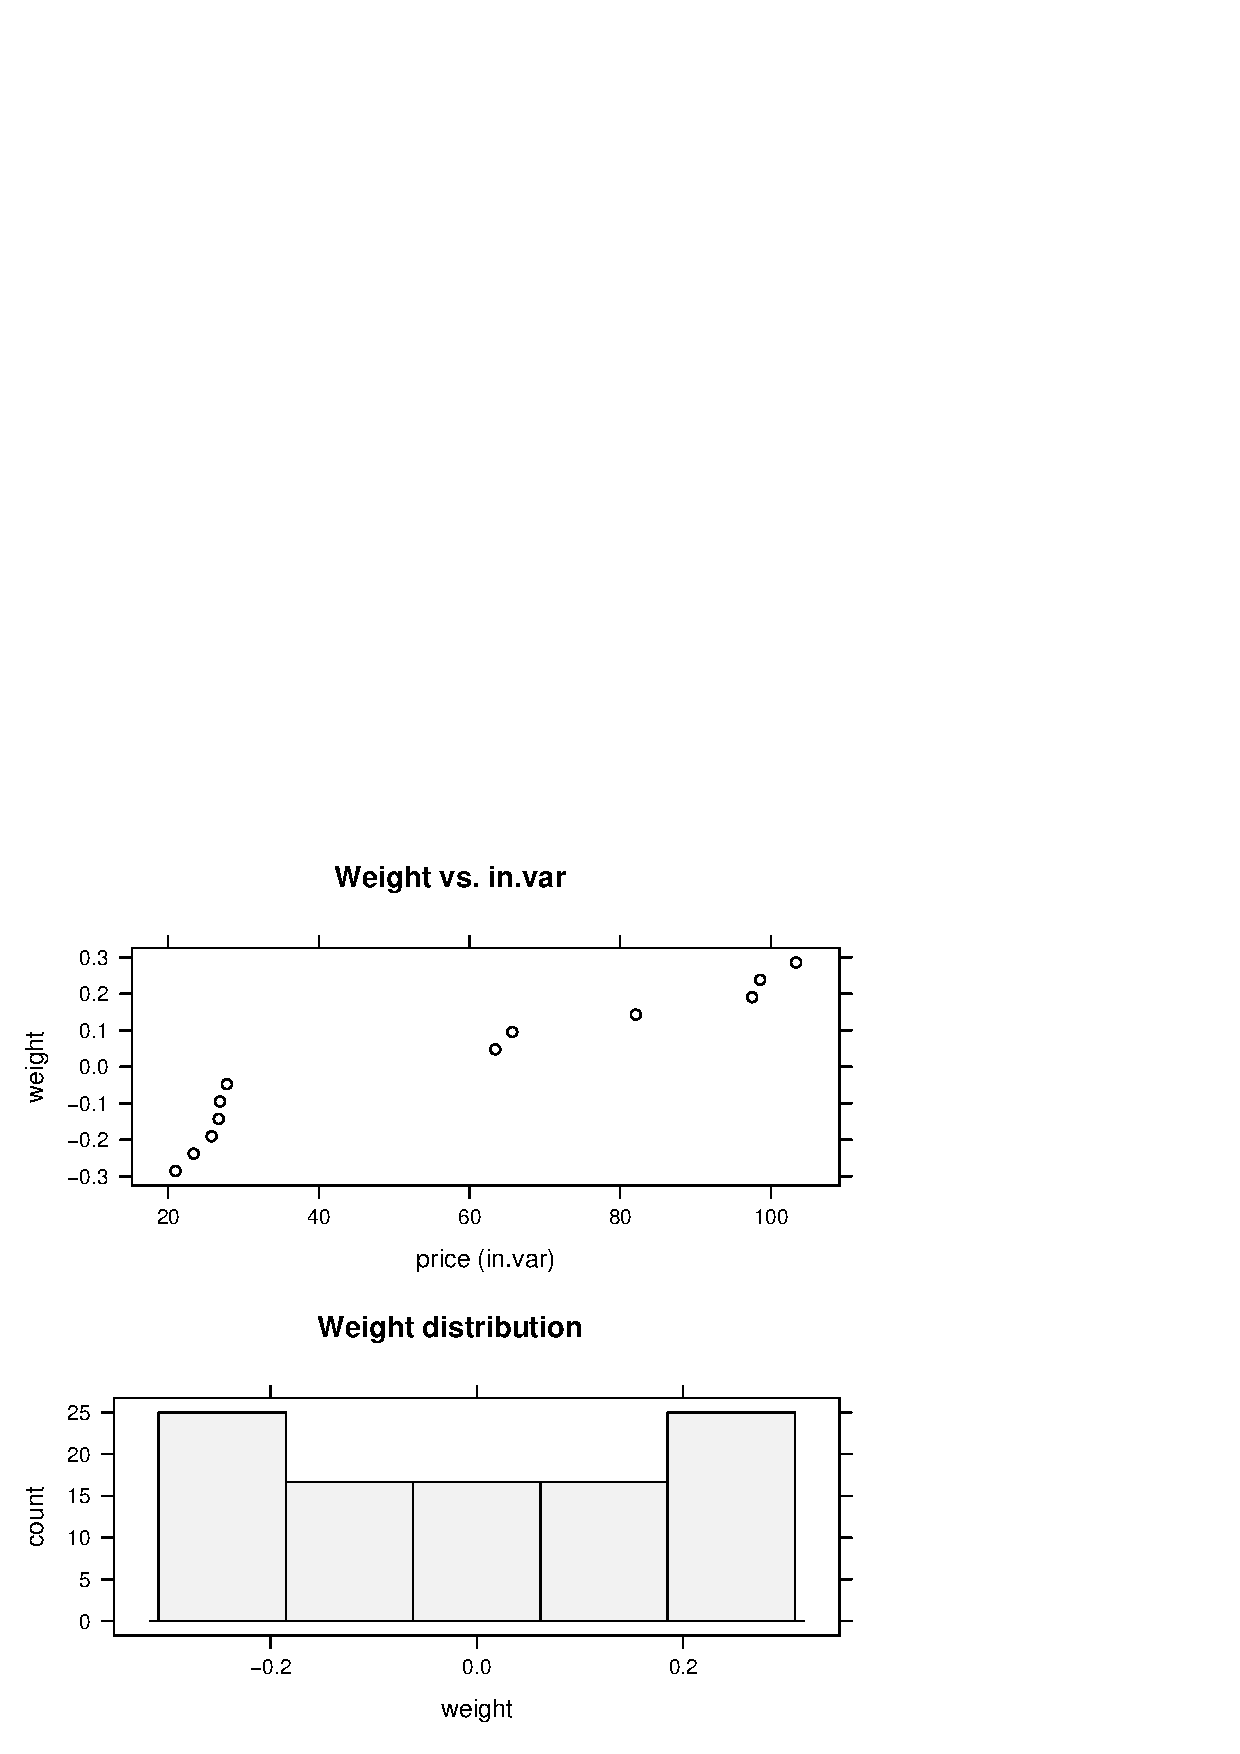
\includegraphics{portfolio-010}
\caption{\label{figure:plot.portfolio}
Plot of a portfolioBasic object.}
\end{figure}

The display for the exposure object is now somewhat different to
accommodate the structure of a long-short portfolio. 

\begin{Schunk}
\begin{Sinput}
> exposure(p, exp.var = c("price", "sector"))
\end{Sinput}
\begin{Soutput}
numeric 
  variable long short exposure
1    price 92.6 -24.2     68.4

sector 
        variable   long   short exposure
2    Industrials 0.6190  0.0000   0.6190
1     Financials 0.0952  0.0000   0.0952
3        Staples 0.0476 -0.0952  -0.0476
5 Communications 0.0000 -0.2381  -0.2381
4     Technology 0.2381 -0.6667  -0.4286
\end{Soutput}
\end{Schunk}

The \texttt{long} exposure to price is simply the weighted average of
price on the long side of the portfolio, where the weighting is done
in proportion to the size of the position in each stock. The same is
true on the short side.  Since a linear weighting used here emphasises
the tail of the distribution, the long exposure is greater than the
long exposure of the equal weighted portfolio considered above, \$93
versus \$85.

Since the weights on the short side are actually negative --- in the
sense that we are negatively exposed to positive price changes in
these stocks --- the weighted average on the short side for a positive
variable like price is also negative.  Another way to read this is to
note that the weighted average price on the short side is about \$24
but that the portfolio has a negative exposure to this number because
these positions are all on the short side.

One reason for the convention of using a negative sign for short side
exposures is that doing so makes the overall exposure of the portfolio
into a simple summation of the long and short exposures. (Note the
assumption that the weights on both sides are equal. In future
versions of the \pkg{portfolio} package, we hope to weaken these and
other requirements.) For this portfolio, the overall exposure is 68.
Because the portfolio is long the high priced stocks and short the low
priced ones, the portfolio has a positive exposure to the price
factor. Colloquially, we are ``long price.''

A similar analysis applies to sector exposures. We have 62\% of our
long holdings in Industrials but zero of our short holdings. We are,
therefore, 62\% long Industrials. We have 24\% of the longs holdings
in Technology, but 67\% of the short holdings; so we are 43\% short
Technology.

Calling \texttt{plot} on the exposure object produces a bar chart for
each exposure category, as seen in Figure \ref{figure:plot.exposure}.  Since all
numeric exposures are grouped together, a plot of numeric exposure may
only make sense if all numeric variables are on the same scale.  In
this example, the only numeric exposure we have calculated is that to
\texttt{price}.

\begin{figure}
\centering
\vspace*{.1in}
\begin{Schunk}
\begin{Sinput}
> plot(exposure(p, exp.var = c("price", 
+     "sector")))
\end{Sinput}
\end{Schunk}
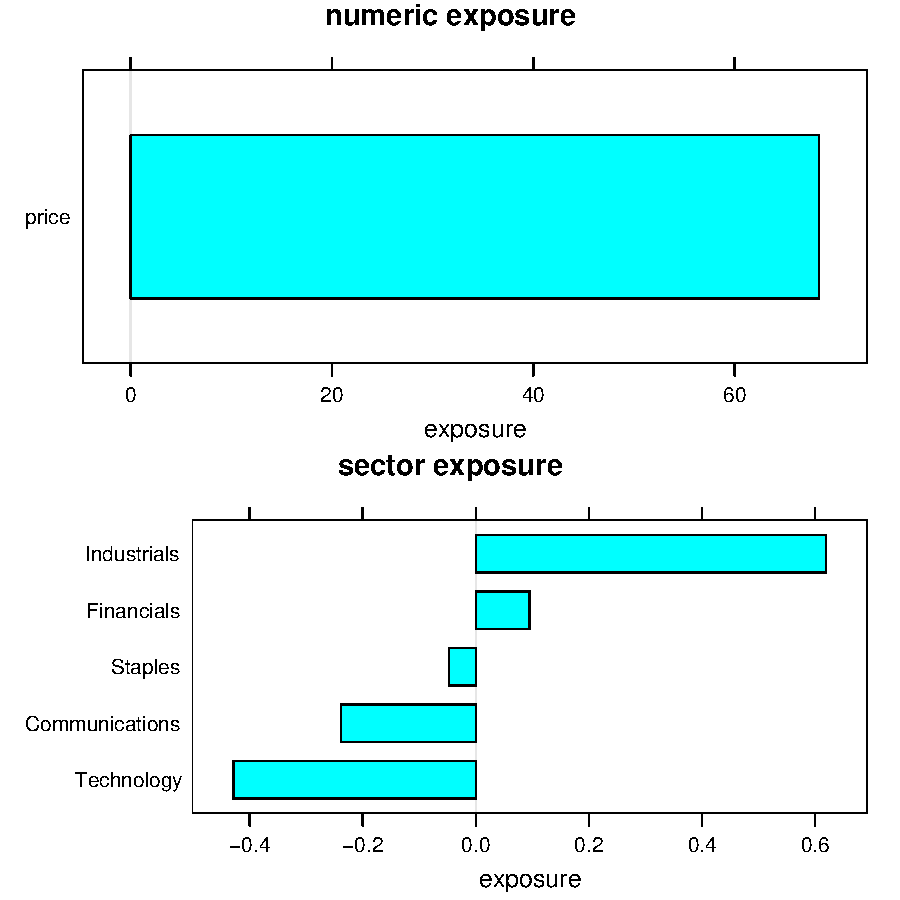
\includegraphics{portfolio-012}
\caption{\label{figure:plot.exposure} Plot of an exposure object for a
single period.  Bar charts are sorted by exposure.}
\end{figure}

The performance object is similar for a long-short portfolio.

\begin{Schunk}
\begin{Sinput}
> performance(p)
\end{Sinput}
\begin{Soutput}
Total return:  2.19 % 

Best/Worst performers:
     id  weight      ret  contrib
2   CAT  0.1905 -0.08220 -0.01566
5   IBM  0.2381 -0.05234 -0.01246
12  UTX  0.2857 -0.02583 -0.00738
3   DIS -0.0476  0.02986 -0.00142
1   AIG  0.0952  0.00944  0.00090
8   MMM  0.1429  0.02790  0.00399
6  INTC -0.2381 -0.04019  0.00957
10  PFE -0.0952 -0.10152  0.00967
11  SBC -0.1905 -0.06617  0.01260
4   HPQ -0.2857 -0.06581  0.01880
\end{Soutput}
\end{Schunk}

The portfolio was up 2.2\% in January. By default, the summary of the
\texttt{performance} object only provides the 5 worst and best
contributions to return. HPQ was the biggest winner because, though it
was only down 7\% for the month, its large weighting caused it to
contribute almost 2\% to overall performance. The 19\% weight of CAT
in the portfolio placed it as only the third largest position on the
long side, but its -8\% return for the month made it the biggest drag
on performance.

The \texttt{contribution} function provides similar output for a
long-short portfolio.

\begin{Schunk}
\begin{Sinput}
> contribution(p, contrib.var = c("cap.bil", 
+     "sector"))
\end{Sinput}
\begin{Soutput}
cap.bil 
      rank    variable weight  contrib     roic
1  1 - low (22.6,50.9] 0.0952 -0.01566 -0.16440
2        2 (50.9,71.1] 0.3810  0.01399  0.03671
3        3  (71.1,131] 0.0952  0.01260  0.13235
4        4   (131,191] 0.3095 -0.00103 -0.00334
5 5 - high   (191,386] 0.1190  0.01202  0.10098

sector 
         variable weight contrib    roic
1  Communications 0.1190  0.0112  0.0939
6   Conglomerates 0.0000  0.0000  0.0000
7       Cyclicals 0.0000  0.0000  0.0000
8          Energy 0.0000  0.0000  0.0000
2      Financials 0.0476  0.0009  0.0189
3     Industrials 0.3095 -0.0191 -0.0616
9       Materials 0.0000  0.0000  0.0000
4         Staples 0.0714  0.0106  0.1488
5      Technology 0.4524  0.0183  0.0404
10      Utilities 0.0000  0.0000  0.0000
\end{Soutput}
\end{Schunk}

As in the last example, the \texttt{weight} column reflects the
proportion of the portfolio invested in each category.  In this case,
we have 45\% of the total capital (or weight) of the long and short
sides \emph{considered together} invested in the Technology sector. We
know from the exposure results above that most of this is invested on
the short side, but in the context of contributions, it does not
matter on which side the capital is deployed.

Plotting objects of class \texttt{contribution} produces output
similar to plotting exposures, as can be seen in Figure
\ref{figure:plot.contribution}.  This time, however, we see values of
\texttt{roic} plotted against the categories that make up each
\texttt{contrib.var}.  For numeric variables, \texttt{roic} for each
interval is shown; numeric intervals will always appear in order.

\begin{figure}
\centering
\vspace*{.1in}
\begin{Schunk}
\begin{Sinput}
> plot(contribution(p, contrib.var = c("cap.bil", 
+     "sector")))
\end{Sinput}
\end{Schunk}
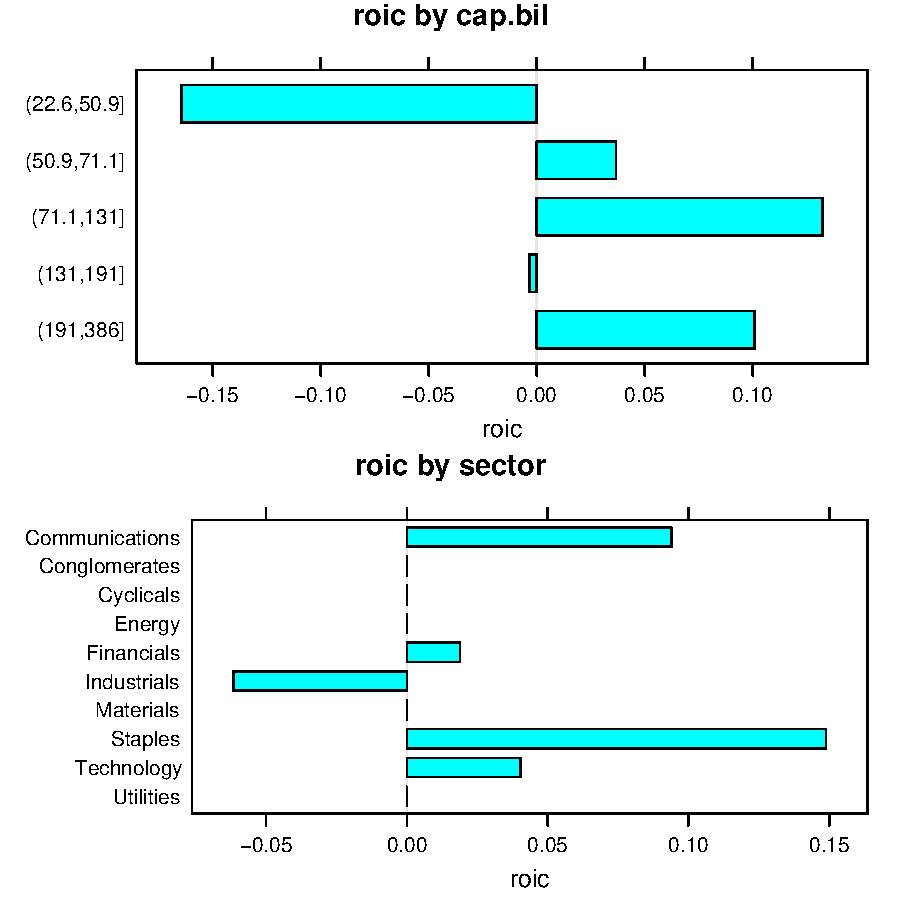
\includegraphics{portfolio-015}
\caption{\label{figure:plot.contribution} Plot of a contribution object for a
single period.}
\end{figure}

\section*{Conclusion}

The current release of the portfolio package is meant to serve as a
proof-of-concept. Relatively sophisticated portfolio analytics are
possible using an open source package. Although money management is
largely a zero-sum game --- every dollar that I make is a dollar that
someone else has lost --- there is no reason why we might not
cooperate on the tools that we all use.

\address{David Kane and Jeff Enos\\
 Kane Capital Management, Cambridge, Massachusetts, USA\\
 \email{david@kanecap.com} and  \email{jeff@kanecap.com}}
\end{article}
\end{document}

